\documentclass[main.tex]{subfiles}
\begin{document}
	
\verb|https://www.spyder-ide.org|

Python software installation:

\verb|https://code.visualstudio.com/Anaconda|: Spyder, Jupiter
集成开发环境(IDE - Integrated Development Environment)\index{集成开发环境 IDE}
Visual Studio Code

PyCharm

\begin{figure}[h]
	\centering
	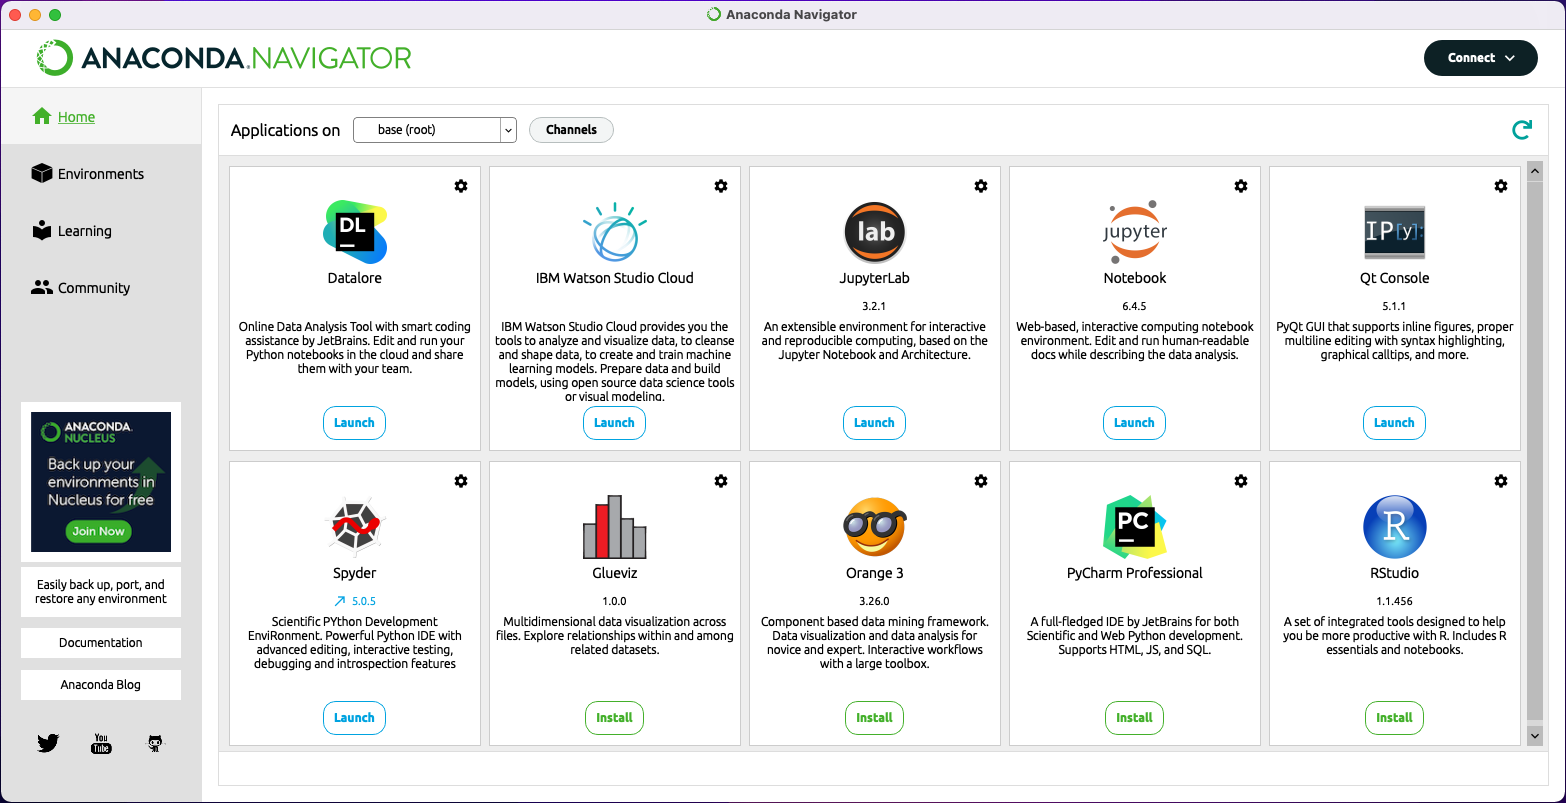
\includegraphics[width=1.0\textwidth]{png/anaconda_navig.png}
	\caption{Anaconda Navigator}
	\label{fig:III.1.3}
\end{figure}


微软公司的视窗操作系统的主要开发语言是C\#,其 IDE 是 Microsoft Visual Studio ${}^{\textregistered}$。但他们也有一个免费的轻巧 IDE,叫做 Visual Studio Code,有 Windows, Linux and macOS 版本,支持 Python,Java,JavaScript,Go,Node.js 和 C++ 等语言。可从
https://code.visualstudio.com
下载的安装。


\end{document} 
